
% !TeX document-id = {d8b4925c-2057-42a4-b894-2f1a3f1b6345}
%!TeX TXS-program:compile = txs:///xelatex/[--shell-escape]
\documentclass[aspectratio=169, mathserif]{beamer}% TPU recommends 16:9 ratio, 4:3 may require some work with inner theme .sty file

% Style options:
% light --- light theme (default)
% dark --- dark theme
% enlogo --- english TPU logo {default}
% rulogo --- russian TPU logo

\usetheme[light, rulogo]{tpu}% dark theme used as an example of optional argument

\usepackage[russian]{babel}%uncomment this to work in russian
\usepackage[utf8]{inputenc}

\usepackage{amsmath}

\usepackage{fontspec}

\setromanfont{Brygada1918}[
Path=./fonts/BrygadaFontFiles/,
Extension = .ttf,
UprightFont=*-Regular,
BoldFont=*-Bold,
ItalicFont=*-Italic,
BoldItalicFont=*-BoldItalic
]

\setsansfont{ALSSirius}[
Path=./fonts/ALSSiriusFiles/,
Extension = .otf,
UprightFont=*-Regular,
BoldFont=*-Bold,
%ItalicFont=*-Italic,
%BoldItalicFont=*-BoldItalic
]

\setmonofont{Consolas}[
Path=./fonts/ConsolasFontFiles/,
%Scale=0.85,
Extension = .ttf,
UprightFont=*-Regular,
BoldFont=*-Bold,
ItalicFont=*-Italic,
BoldItalicFont=*-BoldItalic
]

\usepackage[cache=false]{minted}
\usepackage{xcolor} % to access the named colour LightGray
\usepackage{colortbl}
\definecolor{LightGray}{gray}{0.9}
\definecolor{onedarkBckGr}{RGB}{40, 44, 52}

\usemintedstyle[python]{default}
\setminted[python]{
fontsize=\scriptsize,
escapeinside=||,
mathescape=true,
numbersep=5pt,
gobble=2,
linenos=true,
frame=leftline,
framesep=1mm,
python3=true,
%bgcolor=backcolour,
}

\usemintedstyle[pycon]{default}
\setminted[pycon]{
	fontsize=\scriptsize,
	escapeinside=||,
	mathescape=true,
	numbersep=5pt,
	gobble=2,
	frame=single,
	framesep=1mm,
	python3=true,
%	bgcolor=backcolour,
	linenos=true,
}

\newmint{python}{}

\usepackage{booktabs}% good looking tables
\usepackage{multicol}% text in multiple columns, useful for side-by-side text and pictures
\usepackage{hyperref}
\definecolor{maroon}{cmyk}{0, 0.87, 0.68, 0.32}
\definecolor{halfgray}{gray}{0.55}
\definecolor{ipython_frame}{RGB}{207, 207, 207}
\definecolor{ipython_bg}{RGB}{247, 247, 247}
\definecolor{ipython_red}{RGB}{186, 33, 33}
\definecolor{ipython_green}{RGB}{0, 128, 0}
\definecolor{ipython_cyan}{RGB}{64, 128, 128}
\definecolor{ipython_purple}{RGB}{170, 34, 255}
\definecolor{linkcolor}{HTML}{0000FF} % цвет гиперссылок
\definecolor{urlcolor}{HTML}{800080} % цвет ссылок
\definecolor{backcolour}{rgb}{0.95,0.95,0.92}

\usepackage{longtable}
\usepackage{wrapfig}
\usepackage{ragged2e}
\usepackage[nooneline]{caption}
\DeclareCaptionTextFormat{center}{\centering{#1}}
\captionsetup[table]{justification=raggedleft,
labelformat=empty,
labelsep=endash,
textformat=center,
position=top,
skip=5pt
}

\hyphenpenalty=10000% i don’t think hyphenation in presentations is a good idea, feel free to change however you like

\usepackage{chemfig}

\includeonlyframes{c}

\title{\LARGE{Системный анализ процессов химической технологии}}
\subtitle{\textcolor{tpugreen}{\textbf{Лекция №10}} \\ \textbf{Расчет октановых чисел смешения}}
\author[]{Вячеслав Алексеевич Чузлов, \\
к.т.н., доцент ОХИ ИШПР}
\date{\today}

\begin{document}


% notice usage of \titleframe and several other unconventional functions
% the reason being is custom backgrounds on these slides

\titleframe% title

%\tocframe{}% this custom frame accepts options for ToC


\section{Расчет октанового числа}
\sectionframe

\begin{frame}[fragile, label=c]{Октанвое число}
\scriptsize
\textcolor{tpugreen}{\textbf{Октановое число}}~-- это условная величина, характеризующая детонационную стойкость и численно равная процентному содержанию изооктана в эталонной смеси с н-гептаном, которая по детонационной стойкости эквивалентна испытуемому топливу в условиях стандартного одноцилиндрового двигателя.
\vfill
\centering{\textbf{Эталонные углеводороды}}
\vfill
\begin{minipage}{.48\textwidth}
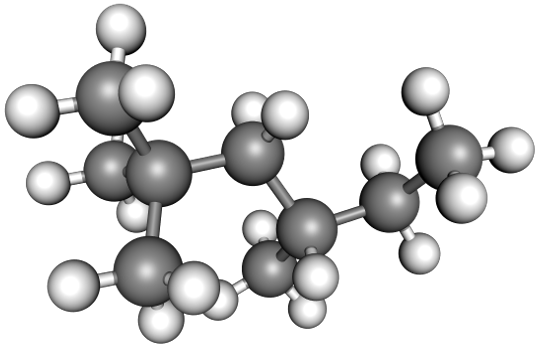
\includegraphics[width=.95\linewidth]{./pics/ic8}
\centering 2,2,4-триметилпентан (изооктан)
\end{minipage}
\begin{minipage}{.01\textwidth}
\hfill
\end{minipage}
\begin{minipage}{.48\textwidth}
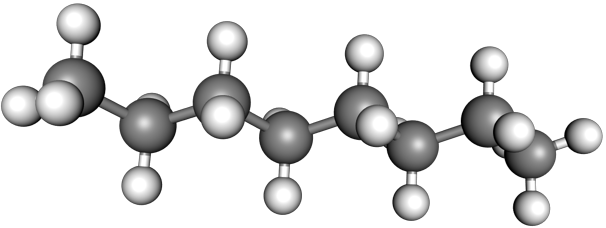
\includegraphics[width=\linewidth]{./pics/nc7}
\centering н-гептан
\end{minipage}
\vfill
\end{frame}



\section{Метод SLSQP}
\begin{frame}[fragile, label=c]{Метод SLSQP}
\scriptsize
\begin{itemize}
\item Метод SLSQP использует последовательное квадратичное программирование для минимизации функций нескольких переменных с любой комбинацией границ, а также ограничений на равенство и неравенство.
\item Метод включает в себя подпрограмму оптимизации SLSQP, первоначально реализованную Дитером Крафтом (Dieter Kraft).
\item Обратите внимание, что оболочка обрабатывает бесконечные значения в границах, преобразуя их в большие значения с плавающей точкой.
\end{itemize}
\vfill
Метод SLSQP работает с задачей минимизации с ограничениями в следующей форме:
\vfill
\begin{equation}\label{eq:problem}
\begin{gathered}
\underset{x}{\min}\ f\left(x\right) \\
\mathrm{при }\ c_j\left(x\right) = 0, \qquad j \in \mathcal{E} \\
\qquad c_j\left(x\right) \geqslant 0, \qquad j \in \mathcal{I} \\
\qquad lb_i \leqslant x_i \leqslant ub_i, \qquad i = 1, \ldots , N.
\end{gathered}
\end{equation}
\vfill
Здесь $\mathcal{E}$ и $\mathcal{I}$~--множества индексов, содержащих ограничения по равенству и неравенству.
\vfill
\end{frame}


\begin{frame}[fragile, label=c]{Метод SLSQP}
\scriptsize
\mintinline[fontsize=\small]{python}|scipy.optimize.minimize(method='SLSQP')|
\vfill
\textbf{Основные параметры:}
\vfill
\begin{itemize}
\item[] \mintinline{python}|fun: callable|

Объектная функция для минимизации.
\vfill
\mintinline{python}|fun(x, *args) -> float|

где \texttt{x}~-- одномерный массив размера \mintinline{python}|(n, )|; \texttt{args}~-- кортеж параметров, необходимых для вызова функции.
\vfill
\item[] \mintinline{python}|x0: ndarray, shape (n,)|

Начальное приближение. Массив элементов размера \mintinline{python}|(n,)|, где \texttt{n}~-- количество независимых переменных.
\vfill
\item[] \mintinline{python}|args: tuple, optional|

Дополнительные аргументы, передаваемые объектной функции и ее производным (функциям \texttt{fun}, \texttt{jac} и \texttt{hess})
\vfill
\item[] \mintinline{python}|bounds: sequence, optional|

Предельные значения для переменных.
\vfill
\item[] \mintinline{python}|constraints: {Constraint, dict} or List of {Constraint, dict}, optional|

Описание функций, накладывающих ограничения на решение.
\end{itemize}
\vfill
\end{frame}


\begin{frame}[fragile, label=c]{Пример}
\scriptsize
\begin{minipage}{.52\textwidth}
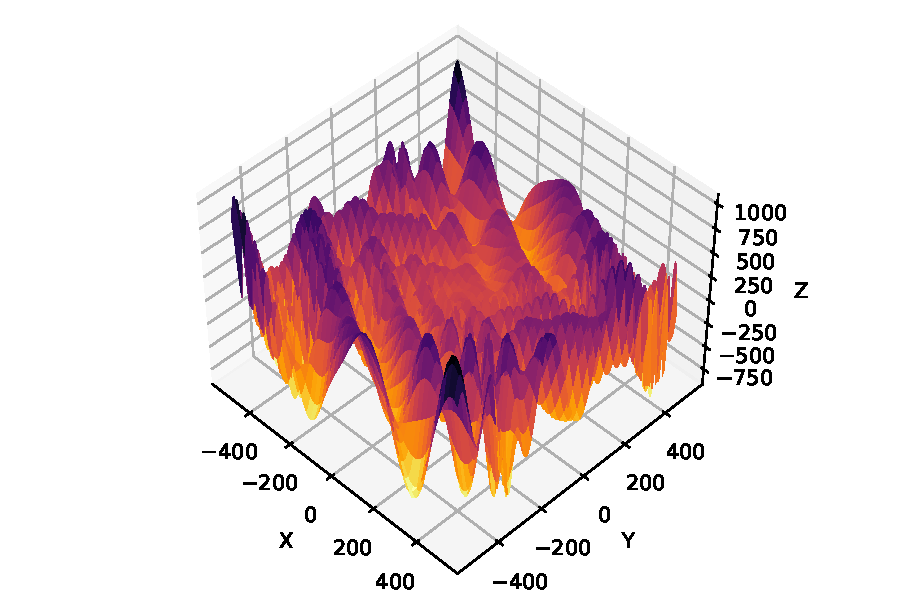
\includegraphics[width=.9\linewidth]{./pics/eggholder}
\end{minipage}
\begin{minipage}{.47\textwidth}
Рассмотрим следующую функцию:
\vfill
\begin{equation*}
z = \left(-y + 47\right) \cdot \sin \sqrt{\left|\dfrac{x}{2} + y + 47\right|} - x \cdot \sin \sqrt{\left|\dfrac{x}{2} - y - 47\right|}
\end{equation*}
\vfill
Найдем минимум данной функции при значениях $x \in \left[400, 500\right];\ y \in \left[400, 500\right]$ и при условии, что $x = y$.
\end{minipage}
\vfill
\end{frame}


\begin{frame}[fragile, label=c]{Пример}
\scriptsize
\begin{minted}{python}
import numpy as np
import scipy.optimize as opt


def func(x):
    return (
        (-x[1] + 47) * np.sin(np.sqrt(abs(x[0] / 2 + x[1] + 47)))
        - x[0] * np.sin(np.sqrt(abs(x[0] - x[1] - 47)))
    )


x = np.arange(-512, 513)
y = np.arange(-512, 513)
xgrid, ygrid = np.meshgrid(x, y)
xy = np.stack([xgrid, ygrid])

bounds = (400, 500), (400, 500)
constr = {
    'type': 'eq',
    'fun': lambda x: x[0] - x[1]
}
\end{minted}
\vfill
\end{frame}


\begin{frame}[fragile, label=c]{Пример}
\scriptsize
\begin{minted}[firstnumber=last]{python}
|\space|
|\space|
res = opt.minimize(
    eggholder,
    x0=(450, 450),
    bounds=bounds,
    constraints=constr,
    method='SLSQP'
)
print(res)
|\space|
\end{minted}
\vfill
\begin{minted}[frame=none, linenos=false]{pycon}
     fun: -641.3734202306166
     jac: array([ 27.49101257, -27.49103546])
 message: 'Optimization terminated successfully'
    nfev: 12
     nit: 4
    njev: 4
  status: 0
 success: True
       x: array([448.93802864, 448.93802864])
\end{minted}
\vfill
\end{frame}



\contactsframe[\Large \textbf{Благодарю за внимание!}]{


\includegraphics[width=.05\textwidth]{pics/home} \quad Учебный корпус №2, ауд. 136 \\

\includegraphics[width=.05\textwidth]{pics/mail} \quad chuva@tpu.ru \\

\includegraphics[width=.03\textwidth]{pics/tel} \quad +7-962-782-66-15
}

\end{document}

